% !TEX root = ../main.tex

\section{Introduction}
\label{sec:introduction}


Recent work on understanding the internal mechanisms of representation learning has brought to attention the problem of shortcut learning~\citep{robinson2021can, chen2021intriguing, scimeca2022which}.
While there are multiple definitions of shortcut learning \citep[e.g., ][]{geirhos2020shortcut, wiles_2022_afinegrained}, in this work we define \emph{shortcuts} as \emph{easy-to-learn discriminatory features that minimize the (contrastive) optimization objective but are not necessarily sufficient for solving the evaluation task}. 
More specifically, we focus on the problem of shortcut learning in the relatively unexplored context of \ac{VL} representation learning with multiple matching captions per image.

\Ac{CL} plays a crucial role in \ac{VL} representation learning. 
Despite the success of non-contrastive approaches, e.g., \citep{bardes2022vicreg}, the dominant paradigm in \ac{VL} representation learning revolves around either fully contrastive strategies~\citep{faghri2018improving, li2019visual, jia2021scaling, radford2021learning} or a combination of contrastive methods with additional objectives~\citep{li2021align, zeng2022multi, li2022blip, zeng2022multi, li2023blip}.
It is standard practice in contrastive \ac{VL} representation learning to sample batches of image-caption pairs and maximize the alignment between the representations of the matching images and captions \citep{radford2019language, jia2021scaling}. 
Given that the typical \ac{VL} benchmarks, e.g., \acl{Flickr30k}\acused{Flickr30k}~\citep{young2014image} and \acl{MS-COCO}\acused{MS-COCO}~\citep{lin2014microsoft, chen2015microsoft}, are constructed in such a way that each image is associated with multiple captions, each caption can be seen as a different \textit{view} of the image it describes. 
Therefore, \ac{CL} with multiple captions per image can be seen as \ac{CL} with multiple views, where each caption provides a different view of the scene depicted in the image.

\Ac{CL} with multiple views, where each view represents a different observation of the same datapoint, has proven to be effective for general-purpose representation learning~\citep{hjelm2019learning, chen2020simple, tian2020contrastive}.
The goal of multi-view (contrastive) representation learning methods is to learn representations that remain invariant to a shift of view, which is achieved by maximizing alignment between embeddings of similar views. 
A core assumption within the multi-view representation learning literature is that task-relevant information is shared across views whereas task-irrelevant information is not shared, given a downstream evaluation task~\citep{zhao2017multi, federici2020learning, tian2020contrastive, shwartz2023compress}.

\begin{wrapfigure}[27]{r}{0.4\textwidth}
	\centering
	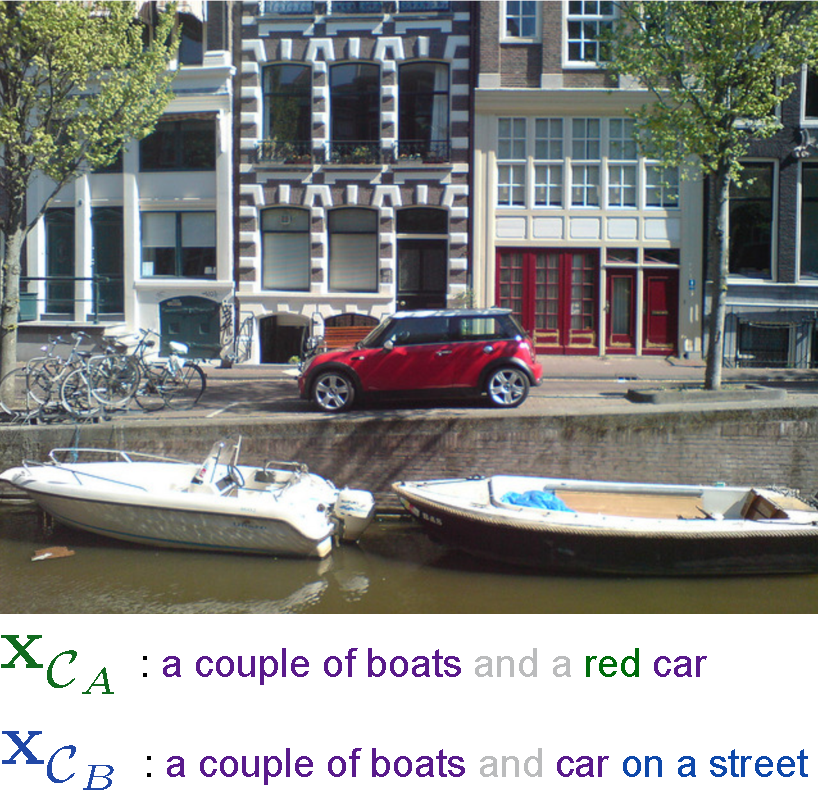
\includegraphics[width=0.4\textwidth]{figures/shared-vs-unique-v2}
	\caption{
	Shared vs. caption-specific information given an example of one image and two associated captions $\capt{}{A}$ and $\capt{}{B}$.
	The purple color indicates information shared between the image and both captions.
	The green color indicates task-relevant information specific for $\capt{}{A}$.
	The blue color indicates task-relevant information specific for $\capt{}{B}$.
	}
	\label{fig:shared-vs-specific}
\end{wrapfigure}

An open challenge in the multi-view representation learning domain concerns \emph{learning representations that contain task-relevant information that is not shared among different views, i.e., that may be unique for some views}~\citep{shwartz2023compress, zong2023self}.
In the case of image-caption datasets where each image is paired with at least one corresponding caption, the captions matching the same image do not necessarily share the same information as each caption is distinct and may describe different aspects of the image~\citep{biten2022_is}.
Figure~\ref{fig:shared-vs-specific} illustrates the concept of shared vs.\ caption-specific task-relevant information.
The image is accompanied by two captions: `a couple of boats and a red car' ($\capt{}{A}$) and `a couple of boats and a car on a street' ($\capt{}{B}$).
The shared information between the captions includes `couple of boats' and `car'.
Caption $\capt{}{A}$ provides unique information by describing the car as `red'. Caption $\capt{}{B}$ adds unique contextual details about the location with the phrase `on a street'.
To learn task-optimal representations, it is essential to integrate both the shared and unique information from these captions.
Furthermore, given the typical quality of captions of image-caption datasets~\citep{chen2015microsoft}, we assume that all information present in the captions is relevant.
Hence, each image-caption pair may contain both \emph{shared} task-relevant information, i.e., information shared across all the captions in the tuple, and \emph{unique} task-relevant information, i.e., information not shared with other captions.
Therefore, learning task-optimal representations for the image implies learning all task-relevant information that comprises both shared and caption-specific information.

Another problem of \ac{CL} approaches is related to \emph{feature suppression}. 
\cite{shwartz2023compress} argue that although contrastive loss functions lack explicit information-theoretical constraints aimed at suppressing non-shared information among views, the learning algorithm benefits from simplifying representations by suppressing features from the input data that are not relevant for minimizing the contrastive loss.
Furthermore, \citet{robinson2021can} demonstrate that contrastive loss functions are susceptible to solutions that suppress features from the input data.
In the case of \ac{VL}, \ac{CL} with multiple captions per image where at least one caption contains caption-specific information, the image representation can never have a perfect alignment with all matching captions.
This is due to the misalignment that happens when encoding unique information for the other captions.
Therefore, it is unclear whether contrastive methods can learn task-optimal representations, i.e., representations that contain all information present in the captions associated with the image, or if they learn only the minimal shared information, i.e., information shared between the image and all captions that are sufficient to minimize the contrastive discrimination objective. 
An illustration of minimal shared information and a task-optimal representation is given in Figure~\ref{fig:latent_viz}. 

% !TEX root = ../../main.tex

\begin{figure*}[t!]
	\centering
	\begin{subfigure}[t]{0.37\textwidth}
		\centering
		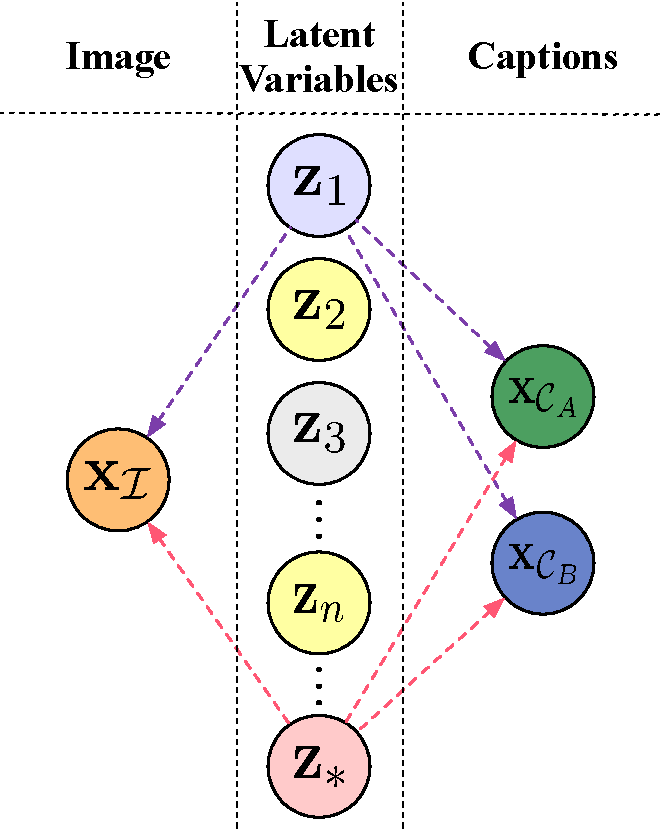
\includegraphics[width=0.75\textwidth]{figures/latent_viz/minimal-shared-representation.pdf}
		\caption{Minimal shared information.}
	\end{subfigure}%
	\qquad
	\begin{subfigure}[t]{0.37\textwidth}
		\centering
		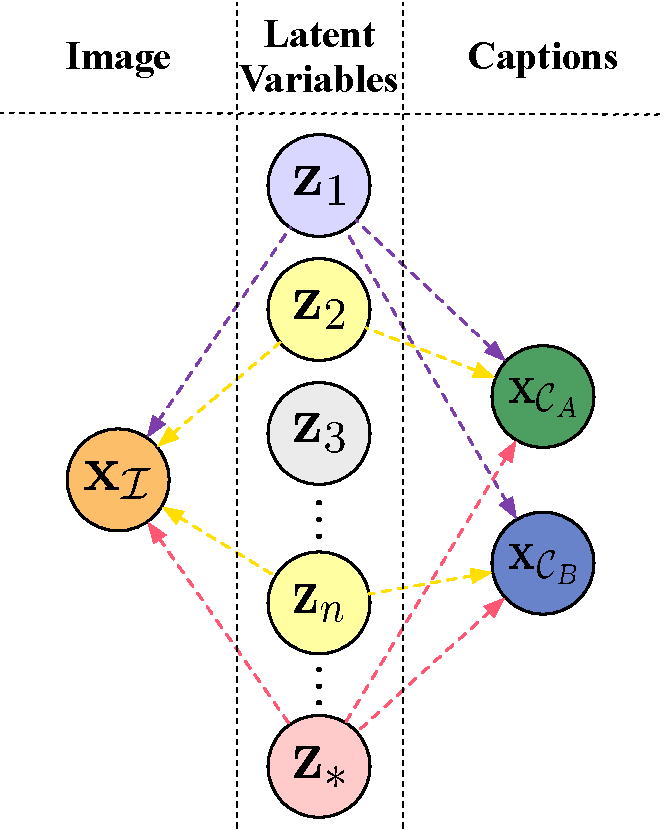
\includegraphics[width=0.75\textwidth]{figures/latent_viz/task-optimal-representation.pdf}
		\caption{Task-optimal information.}
	\end{subfigure}
	\caption{
	Synthetic shortcuts in the context of minimal shared and task-optimal information for vision-language representation learning with multiple captions per image. 
        The purple color represents features shared among the image and all captions (minimal shared information).
        The yellow color represents caption-specific features (unique information).
        The grey color indicates features that are not present in both the image and any of the captions (task-irrelevant information).
        The red color indicates synthetic shortcuts. 
        We demonstrate that while shortcuts exist in both scenarios, minimal shared information also includes information shared among the image and all associated captions, whereas task-optimal information combines both minimal shared information and caption-specific information.
	}
	\label{fig:latent_viz}
\end{figure*}  

Motivated by the abovementioned problems, we address the following question:
\begin{quote}
\emph{In the context of \ac{VL} representation learning with multiple captions per image, to what extent does the presence of a shortcut hinder learning task-optimal representations?}
\end{quote}

To answer this question, we investigate the problem of shortcut learning for \ac{VL} representation learning with multiple captions per image.
We do this by introducing the \acfi{SVL} framework for adding additional, easily identifiable information to image-caption tuples. 
The information that we add is represented as identifiers that are applied to both image and caption; these identifiers do not bear any semantic meaning. 
The identifiers provide additional shared information between the image and captions, which is a subset of the total shared information between the image and the caption.
For details and examples of shortcuts, refer to Section~\ref{eval:method}, where Figure~\ref{fig:shortcut-example} illustrates an example of an image-caption pair with a shortcut added.
The synthetic shortcuts framework allows us to investigate how much the encoder model relies on the added shortcut during training and evaluation, and hence how much of the relevant information is still captured if a shortcut solution is available.
Overall, our \ac{SVL} framework allows us to investigate the shortcut learning problem in a controlled way. 
We focus on \ac{ICR} as an evaluation task because contrastive losses directly optimize for the \ac{ICR} evaluation task, which assesses the quality of the learned representations by computing a similarity score between images and captions~\citep{radford2021learning, yuksekgonul2023when}.
To investigate the problem, we run experiments on two distinct models:
\begin{enumerate*}[label=(\roman*)]
	\item CLIP~\citep{radford2019language}, a large-scale model that we fine-tune; and
	\item VSE++~\citep{faghri2018improving}, a relatively small model that we train from scratch.
\end{enumerate*}
We evaluate the models' performance on the \ac{Flickr30k}~\citep{young2014image} and \ac{MS-COCO}~\citep{lin2014microsoft, chen2015microsoft} and benchmarks. 
The benchmarks are constructed in such a way that each image is associated with five captions and each caption represents a concise summary of the corresponding image.

Therefore, the contributions of this work are two-fold: 
\begin{enumerate}[label=\Roman*]
	\item \textbf{A framework for investigating the problem of shortcut learning for contrastive \acl{VL} representation learning in a controlled way}:
	We introduce the \textit{\acl{SVL}} framework.
	The framework enables the injection of synthetic shortcuts into image-caption tuples in the training dataset. 
	We use the framework to investigate and understand the extent to which contrastive \ac{VL} models rely on shortcuts when a shortcut solution is available. 
	We run our experiments using CLIP and VSE++, two distinct \acp{VLM}. We evaluate the models' performance on the \ac{Flickr30k} and \ac{MS-COCO} benchmarks.
	We evaluate the effectiveness of contrastive \ac{VL} models by comparing their performance with and without synthetic shortcuts.
	We demonstrate that both models trained from scratch and fine-tuned, large-scale pre-trained foundation models mainly rely on shortcut features and do not learn task-optimal representations.
	Consequently, we show that contrastive losses mainly capture the easy-to-learn discriminatory features that are shared among the image and all matching captions, while suppressing other task-relevant information. 
	Hence, we argue that contrastive losses are not sufficient to learn task-optimal representations for \ac{VL} representation learning.
	\item \textbf{We present two shortcut learning reduction methods on our proposed training and evaluation framework:}  We investigate \acf{LTD} and \acf{IFM} using our \ac{SVL} training and evaluation framework. 
	While both methods improve performance on the evaluation task, our framework poses challenges that existing shortcut reduction techniques can only partially address, as the performance is not on par with models trained without synthetic shortcuts.
	These findings underline the importance and complexity of our framework in studying and evaluating shortcut learning within the context of contrastive VL representation learning.
\end{enumerate}
